\lhead{\emph{Methods}} % This is for the header on each page - perhaps a shortened title
\label{chpt:modelling and techniques}

This chapter describes in detail the two modelling techniques used for this thesis: the characterisation of a CV using multi-band eclipse modelling, and using MESA models to infer the long-term mass loss rate of a system from its donor properties.
Since the models used in this analysis are computationally expensive and require large parameter spaces, the choice of fitting algorithm is important. The majority of the parameter optimisation done in this work uses a type of Markhov Chain Monte Carlo (MCMC) technique, and this is described in detail in \S\ref{sect:modelling:parameter optimisation of many variables}, before discussing the models themselves.


\section{Parameter optimisation of many variables}
\label{sect:modelling:parameter optimisation of many variables}
Frequently in science, a model must have its input parameters fit to data. For models with few input parameters and well-behaved evaluation metrics (i.e. goodness-of-fit varies smoothly with input parameters), optimisation is relatively easy, but this is often not the case; for example the eclipse modelling portion of this work (\S\ref{sect:modelling:eclipse modelling}) has 18 parameters for a single eclipse, and fitting a full dataset frequently involves fitting  100+ parameters. To make matters worse, the eclipse model is fairly expensive to compute in large numbers, making a full exploration of the parameter space impractical.

The MCMC method is now a well-established tool in astronomy. It is robust, efficient when used properly, and yields the probability distribution of the variables being optimised even when the distributions are not well-described by simple functions. This has led to MCMC often being the method of choice when fitting models.
This section provides a working knowledge of MCMC, but for an in-depth introduction and review of the technique and its various sub-types see \citet{sharma2017}.


\subsection{Bayesian analysis}
\label{sect:modelling:Bayesian analysis}
Bayesian inference uses known, `prior' knowledge combined with new information, `data', to derive a better understanding - the `posterior' knowledge - of a model. This somewhat self-evident intuition is formalised as Bayes' Theorem, which calculates the posterior probability, $p(\theta | D, I)$ a set of model parameters, $\theta$, given some observed data, $D$, and background information, $I$.
\begin{equation}
    \label{eqn:modelling:bayes symbolic}
    p(\theta | D,I) = \frac{\mathcal{L}(D | \theta, I) \cdot q(\theta | I)}{p(D|I)}
\end{equation}
Here, $\mathcal{L}(D | \theta, I)$ is the probability of the observed data, given a model and prior information, so is called the likelihood of the data.
$q(\theta|I)$ is the probability of the model being valid, given some prior information, so is called the prior distribution. Finally, $p(D | I)$, or the probability of observing the data, given the previously known information, is also called the `Evidence', and acts as a normalisation factor. Using this vocabulary, Equation~\ref{eqn:modelling:bayes symbolic} can be written as:
\begin{equation}
    \label{eqn:modelling:bayes english}
    \rm Posterior = \frac{Likelihood \times Prior}{Evidence}
\end{equation}
In Bayesian inference, the goal is to find the posterior distribution of the parameters of a model, given some data and any prior information.


\subsection{MCMC optimisation}
\label{sect:modelling:affine invariant MCMC}
The MCMC technique is a class of tools developed to approximate the posterior distribution in Equation~\ref{eqn:modelling:bayes symbolic}. Analytical calculations of the posterior are predicated on knowing the analytical forms of the likelihood, prior and evidence, which is often not known.

An MCMC sampler, as the name suggests, is a combination of a Monte Carlo method, a class of algorithms that rely on random sampling to find a result, and a Markov chain, a mathematical system that transitions between states according to probabilistic rules \citep{foreman2012}.
An MCMC randomly samples the prior distributions of the model variables (the Monte Carlo half of the algorithm), evaluates their $\mathcal{L}$ and $q$, and either accepts them onto its chain of sampled points or not, depending on if they meet a set of conditions (the Markov chain half of the algorithm). If the $\mathcal{L}$ of the proposed set of variables is higher than the $\mathcal{L}$ of the last set on the chain, the proposed set of variables is accepted. If $\mathcal{L}$ is lower, the algorithm randomly accepts or rejects the proposed step.
Conveniently, $\mathcal{L}$ is usually related to the $\chi^2$ metric by $\mathcal{L} \propto \mathrm{exp}(-\chi^2/2)$, so a change in $\mathcal{L}$ is often relatively easy to compute.
The method by which a new set of parameters is proposed, and acceptance decided in the event of a decrease in $\mathcal{L}$ is the sampling method, and several choices exist for different types of problems. The sampling method used here is the affine invariant sampling method with parallel tempering, described below.

By giving a finite chance to accept a `worse' set of parameters, the chain is, in theory, allowed to explore and sample the entire possible parameter space without becoming trapped in local minima, though this requires an infinitely long chain.
However, as the sampler preferentially accepts positions with higher $\mathcal{L}$, as the length of the chain increases the distribution of samples on the MCMC chain approaches the `true' distribution of the posterior.


\subsubsection{Affine invariant ensemble sampling}
\label{sect:modelling:Affine invariant ensemble sampling}
The affine invariant ensemble method of sampling was developed by \citet{goodman2010}, and makes use of many `walkers' sampling the parameter space in tandem.
Each walker functions as an individual MCMC chain, and the walkers interact by proposing steps based on the current states of other walkers.
A new parameter vector for walker $k$ is proposed via a `stretch move'; another walker, $j$ is chosen at random, and the last position vectors on each chain, $\theta_{j,N}$ and $\theta_{k,N}$, are used to propose a new position, $\Theta_k$, that lies somewhere on the line connecting the two position vectors.
\begin{equation}
    \Theta_k = \theta_j + z \cdot (\theta_k - \theta_j)
\end{equation}
The variable $z$ determines the location of the new vector on the line, and is randomly drawn from a probability distribution $g(z)$,
\begin{equation}
    g(z) \propto
    \begin{cases}
        \frac{1}{\sqrt{z}}, & \frac{1}{2} \le z \le 2 \\
        0, & Otherwise
    \end{cases}
\end{equation}
The choice of $g(z)$ favours a consolidation of the walkers, and aids convergence on regions of high $\mathcal{L}$. A schematic of this stretch move concept is shown in Figure~\ref{fig:modelling:stretch move}.
\begin{figure}
    \centering
    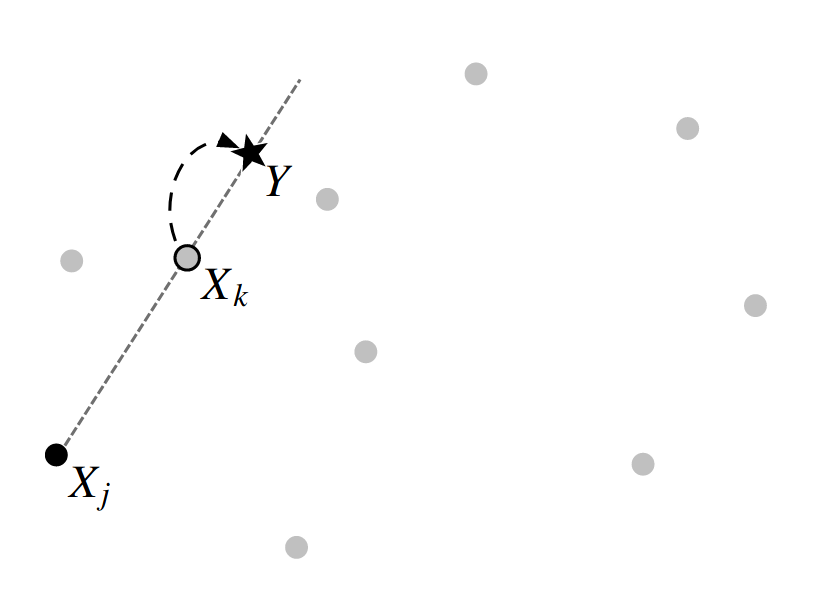
\includegraphics[width=.7\textwidth]{figures/modelling/stretch_move.png}
    \caption{Reproduced from \citet{goodman2010}, showing the concept of a stretch move proposal. The proposed next step for $j$ is given by choosing a random position on the line joining the last step on chain $j$, $X_j$, and the last chain on another walker chosen at random, $X_k$. The proposed step is shown by the star, $Y$. Grey dots with no outlines illustrate the other walkers in the ensemble, but are unused.}
\label{fig:modelling:stretch move}
\end{figure}

Then, $\Theta_k$ is either accepted or rejected from the chain depending on the current state of the chain. Recall that if the proposed $\mathcal{L}_{N+1} > \mathcal{L}_{N}$, i.e. the likelihood has improved, the sample is immediately accepted. However, if $\mathcal{L}_{N+1} < \mathcal{L}_{N}$, the acceptance is determined by the transition probability, $P(\Theta_k | \theta_{k,N})$, defined as
\begin{equation}
    P(\Theta_k | \theta_{k,N}) = \alpha(\Theta_k | \theta_{k,N}) \cdot q(\Theta_k | \theta_{k,N})
\end{equation}
where $\alpha(\Theta_k | \theta_{k,N})$ is the acceptance probability,
\begin{equation}
    \alpha(\Theta_k | \theta_{k,N}) = \mathrm{min}\bigg( 1,\ z^{n-1}\frac{\mathcal{L}(\Theta_k)}{\mathcal{L}(\theta_{k,N})} \bigg)
\end{equation}
for a model with $n$ dimensions.
A random number, $u$, is drawn from a uniform distribution from 0 to 1, and if $u < \alpha(\Theta_k | \theta_{k,N})$, the proposed position is accepted.
This quantifies two aspects of the sampler: the larger the drop in the probability that a new $\Theta_k$ describes observation, the \textit{less likely} the algorithm is to accept $\Theta_k$ onto the chain; and larger stretch moves are more likely to be accepted.
At each step in the MCMC, every walker has a new position proposed this way.

% This finite chance to accept a new point, even if it is less likely to describe the data, makes the chain \textit{reversible} and allows the algorithm to explore the full allowable parameter space (given an infinite number of steps) even if doing so first requires moving to a less preferred $\theta$.
The affine invariant ensemble sampler benefits significantly from having the walkers in the ensemble interact, as they can communicate to other walkers regions of high $\mathcal{L}$ even between walkers in different local minima. Further, the sampler has a higher likelihood to accept dispersing steps than consolidating steps, so walkers are only likely to gather in deep minima, increasing exploration except in the case of a significantly higher likelihood.
This improves the ensemble's ability to both locate the global minimum, and to sample non-spherical probability distributions (a task that can be difficult for simpler sampling techniques).
Further, this algorithm is able to have the proposal and evaluation of new steps in every chain performed \textit{simultaneously}, significantly improving computation time;
a typical rule-of-thumb is to use $2n$ walkers for $n$ parameters being optimised \citet{goodman2010}, and since the number of walkers is almost always larger than the number of available threads, increased evaluation time scales well with more threaded computation.


\subsubsection{Parallel tempering}
\label{sect:modelling:parallel tempering}

Parallel tempering is an additional element of an MCMC sampler that helps in more fully exploring the parameter space in more complex models, while also being more capable of characterising posterior distributions in the case of complex correlations between parameters \citep{earl2005}.

In metallurgy, a metal can be toughened by relieving its internal stresses through tempering, a treatment in which a metal is first heated to a high temperature, then slowly cooled.
While the metal is at a high temperature, impurities are able to diffuse throughout the crystal structure of the metal and explore possible crystallisation locations. As the metal slowly cools, impurity atoms are gradually more and more attracted to areas of the crystal that exert less stress on the material, until the metal is fully cooled and the majority of atoms have found areas of local minima in stress potential.

The ensemble MCMC can take analogy from this `hot' exploration phase and `cool' settling phase \citep{earl2005}. This is done by running several parallel ensembles, that each have a different `temperature' between 1 and $\infty$. Each ensemble samples a modified posterior, that follows $\pi_T(\Theta)$;
\begin{equation}
    \pi_T(\Theta) = [\mathcal{L}(\Theta)^\frac{1}{T}] q(\Theta)
\end{equation}
As $T \rightarrow \infty$, the chain samples the prior with no respect to how well $\Theta$ describes the data. This hot chain is analogous to the diffusive atoms with much higher thermal energy than the stress potential of the metal, and is free to randomly explore available parameter space without being restricted by the $\mathcal{L}$ function, potentially finding regions of high likelihood far from the initial conditions and communicating these regions back to cooler ensembles. Cooler temperatures are analogous to the cooling metal -- drawn increasingly strongly towards regions of high likelihood.
The cold case of $T \equiv 1$ behaves equivalently to a normal ensemble sampler.

Note that because hotter walkers are less sensitive to $\mathcal{L}$, their posterior no longer accurately reflects the `true' distribution. If a parameter is described by a Gaussian distribution with a standard deviation, $\sigma$, the tempered $\mathcal{L}$ will have a standard deviation of $\sigma \sqrt{T}$.

When running a parallel tempered MCMC, the values used in the software are $\beta = 1/T$, for which we choose between 3 and 5 evenly spaced values of $\beta$ between 0 and 1.
The number of temperatures used depends on the evaluation time; since parallel tempering runs multiple full ensembles in tandem, in models with very large numbers of parameters it becomes highly desirable to use as few temperatures as possible. However, the penalty in computation time per step comes with the benefit of a dramatically improved ability to locate the global minimum, especially in complex parameter space.

\subsection{The binary chop}

When searching for the root of a simple model, i.e. one with a single input parameter, $x$, and a single output metric, $y$, that either monotonically increases or decreases with $x$, we use the binary chop algorithm.
This requires relatively few evaluations to find the root of a function, i.e. $y(x_0) = 0$.
If two values of $y$ are known to have opposite signs, e.g. $y_1(x_1)$ is positive and $y_2(x_2)$ is negative, it can be deduced that $x_0$ lies between $x_1$ and $x_2$. Then, by repeatedly evaluating midpoint between the two values of $x$ known to be closest to $x_0$, the algorithm will tend towards $x_1 \sim x_2 \sim x_0$. In practice, the optimisation terminates when $y(x_1) - y(x_2)$ is within some tolerance.
Step-by-step, this proceeds as follows:
\begin{enumerate}
    \setlength\itemsep{0em}
    \item First, evaluate the upper and lower limits of $x$, $x_{\rm low}$ and $x_{\rm high}$, to ensure that one returns a negative $y$, and one returns a positive $y$
    \item Evaluate $y(x_{\rm mid})$, where $x_{\rm mid} = 0.5(x_{\rm low} + x_{\rm high})$.
    \item If $x_{\rm low}$ has the same sign as $x_{\rm high}$, assign $x_{\rm high} = x_{\rm mid}$, or vice-versa for $x_{\rm low}$.
    \item Check if the difference between $y(x_{\rm low})$ and $y(x_{\rm high})$ is within tolerance. If it is, terminate the optimisation. Otherwise, repeat the process again.
\end{enumerate}


\section{Finding an orbital ephemeris}
\label{sect:modelling:getting ephemeris}

Crucial to both observing and modelling an eclipse is a good knowledge of the orbital ephemeris. This is described by the equation
\begin{equation}
    \label{eqn:modelling:general ephemeris equation}
    T_{\rm ecl} = T_0 + P_{\rm orb} E
\end{equation}
where $T_{\rm ecl}$ is the time of mid-eclipse, $T_0$ is the mid-eclipse time of the zeroth eclipse, and $E$ is the eclipse number. Accurately calculating $T_{\rm ecl}$ is important to scheduling observations of a system, and $P_{\rm orb}$ is a crucial to the eclipse modelling.

As observations are often separated by several months or even years, an error in $P_{\rm orb}$ of even $\sim 0.1$ seconds can accumulate to give significantly inaccurate predicted eclipse times. This need for precision also requires the definition of {\it where} a time is recorded from, as the delay introduced by the light travel time from one side of the earth's orbit to the other can significantly offset an observed time. All eclipse times presented in this thesis are given in the Barycentric Modified Julian Date (BMJD), which is the time of eclipse as measured from the centre of mass of the solar system. Note that this is different to the heliocentric MJD often seen in the literature, and where heliocentric literature values are used, they are converted to BMJD.
Two timescales are relevant: UTC, in which a clock ticks at the rate of an earth-bound observer; and TDB, in which a clock ticks at the rate of an observer at the barycentre of the solar system. Literature values, and the clocks in the observing cameras, use UTC time. This is converted to TDB during photometric calibration, for consistency with the BMJD times used.

\subsection{Finding eclipse times}
\label{sect:modelling:finding eclipse times}

When finding an eclipse time, simply taking a time of minimum light is insufficient for the systems in this work. This is because it is common for CV eclipses to have very flat eclipse minima, and because CV eclipses have a fairly complex structure.
Rather, finding the mid-eclipse time is done by looking at the numerical derivative of an eclipse.
First, an eclipse is smoothed to remove short term fluctuations, partly those due to noise but also to mitigate the short term flickering often seen in CVs. This initial smoothing is done by applying a median filter to the data. Then, the numerical derivative is calculated and smoothed again, this time with a `boxcar' convolution (a.k.a. a moving average). Properly filtered, the dominant remaining features of the numerical derivative are the ingresses and egresses of the white dwarf and bright spot.
The white dwarf ingress and egress are, in theory, symmetrical -- the ingress should be a sharp, negative spike, and egress should be a sharp, positive spike. As the two should be the same shape, a double-Gaussian is fit to the derivative, using manually chosen initial conditions. In this model, two Gaussians share a width, $\sigma$, and have their mid-points equidistant from a central point. The magnitude of their heights are shared, but with opposite signs;
\begin{align*}
    T_{\rm 1,2} = T_{\rm ecl} \pm \Delta T \\
    h_{\rm 1,2} = \pm h
\end{align*}
where $T_{1,2}$ are the respective midpoints of the two Gaussians, $h_{1,2}$ are their respective heights, and $2\Delta T$ is the distance between the two Gaussians.
The derivative is then fit with these four free parameters ($T_{\rm ecl},\ h,\ \Delta T,\ \sigma$) using an MCMC with wide, uniform priors of appropriate ranges, to give the $T_{\rm ecl}$.

\subsection{Computing period}
\label{sect:modelling:Computing ephemeris}

To find a rough initial ephemeris of a system, at least two eclipse observations with known $E$ are necessary. Given no prior knowledge of $P_{\rm orb}$ and $T_0$, this can be done by simply observing the system for several hours, until two consecutive eclipses are seen. This gives a rough measure of $P_{\rm orb}$, but can be significantly refined with longer baseline observations.
For each observed $T_\mathrm{ecl}$, $E$ could unambiguously be determined, either from observing consecutive eclipses or from previously reported literature values. Where literature values were used to calculate a value of $E$, the result never deviated from an integer by more than 0.25 and were rounded to the nearest whole number.

An MCMC algorithm was used to fit a straight line model to the independent variable $E$\ and dependent variable $T_\mathrm{ecl}$, with a gradient $P$\ and intercept $T_0$; i.e. model values of $T'_{\rm ecl}$ were generated from the set of $E$ and a proposed $(P, T_0)$ pair, and $(T_{\rm ecl} - T'_{\rm ecl})$ was minimised. Again, wide uniform priors were used for $P$ and $T_0$, based on initial values.

The model also accounts for potential systematic differences in timing accuracy between instruments by having variable error scale factors applied to all eclipses observed with a specific instrument. For example, the timing reported for eclipses observed with ULTRACAM may be systematically offset from reality, and the errors associated with those observations might need to be larger than reported to be consistent with data from other instruments. The prior distribution assumed for these error factors was log-uniform ranging from 0.01 to 5, which favours the smallest error-multiplying factor consistent with the data.

Finally, the values of $E$ for each eclipse were offset to minimise the covariance between $T_0$ and $P$.
Consider a predicted eclipse time for $E$. The uncertainty on $T_{\rm ecl}$ in Equation~\ref{eqn:modelling:general ephemeris equation} can be written as,
\begin{equation}
    \label{eqn:modelling:error in ephemeris}
    \sigma_{T{\rm ecl}}^2 = \sigma_{\rm T0}^2 + 2\sigma_{\rm T0} \sigma_{\rm P}E + \sigma_{\rm P}^2 E^2
\end{equation}
from the standard error propagation formula.
To evaluate an alternative set of $E'$, $E$ can be offset by some integer, $N$, with $E' = E - N$. By substituting this into equation~\ref{eqn:modelling:error in ephemeris}, expanding out the brackets, and consolidating some terms, $\sigma_{T{\rm ecl}}^2$ becomes,
\begin{align*}
    \sigma_{T{\rm ecl}}^2 =& \sigma_{\rm T0}^2 + 2\sigma_{\rm T0} \sigma_{\rm P}(E'+N) + \sigma_{\rm P}^2 (E'+N)^2 \\
    % =& (\sigma_{\rm T0}^2 + \sigma_{\rm P}^2 N^2 + 2\sigma_{\rm T0} \sigma_{\rm P} N) + 2(\sigma_{\rm T0} \sigma_{\rm P} + \sigma_{\rm P}^2 N)E' + \sigma_{\rm P}^2 E'^2
\end{align*}

To minimise the cross-correlation between $P$ and $T_0$, the second term of the above equation should be minimised.
This is achieved by setting $N = -(\sigma_{\rm T0}\sigma_{\rm P})/(\sigma_{\rm P}^2)$, and re-fitting the ephemeris. Then, the above becomes:
\begin{equation}
    \sigma_{T{\rm ecl}}^2 = \sigma_{\rm T0}^4 + (\sigma_{\rm P}E')^2
\end{equation}
with no cross correlation, in theory. In practice, as $E$ must be rounded to an integer, some residual cross-correlation persists, but is minimised.

\newpage
\section{Modelling CV eclipse lightcurves}
\label{sect:modelling:lightcurve modelling}

\begin{table}
    \centering
    \caption{The various symbols used in this chapter, and their meanings.}
    \label{table:modelling:parameter key}
    \begin{tabular}{cl}
        \hline
        Symbol & Parameter \\
        \hline
        \hline
        $F_{\rm wd,\ donor,\ disc, bs}$                                 & White dwarf, donor star, disc, and bright spot fluxes   \\
        $T_{\rm eff}$                                                   & White dwarf effective temperature \\
        log($g$)                                                        & White dwarf surface gravity \\
        $M_{\rm wd}$, $R_{\rm wd}$                                      & White dwarf mass and radius                             \\
        $M_{\rm donor}$, $R_{\rm donor}$                                & Donor star mass and radius                              \\
        $q$                                                             & Mass ratio                                              \\
        $a$                                                             & Orbital separation                                      \\
        $x_{l1}$                                                        & Distance from the white dwarf to the $L_1$ point        \\
        $i$                                                             & inclination                                             \\
        $\Delta \phi$                                                   & White dwarf eclipse width in units of phase             \\
        $R_{\rm disc}$                                                  & Accretion disc radius                                   \\
        $b$                                                             & Disc surface profile exponent                           \\
        $\theta_{\rm yaw}$, $\theta_{\rm tilt}$, $\theta_{\rm az}$      & Bright spot yaw, tilt, azimuth                          \\
        $S$                                                             & Bright spot length scale                                \\
        $Y, Z$                                                          & Bright spot profile exponents                           \\
        $u_{\rm ld}$                                                    & White dwarf limb darkening coefficient                  \\
        $\phi_0$                                                        & An eclipse phase offset                                 \\
        $\pi$                                                           & Parallax                                                \\
        E(B-V)                                                          & Interstellar extinction   \\

        \hline
    \end{tabular}
\end{table}

To determine the system parameters for the CVs in this study, the eclipse light-curves were modelled. This method is more frequently applicable in CVs than the more traditional approach of using spectroscopic eclipsing binaries, since the donor star is rarely directly visible. Compared to using the superhump period excess to estimate the mass ratio \citep{patterson2005, knigge2006}, lightcurve modelling requires few assumptions. However, it does require reasonably precise alignment of the system and so is not possible for a large fraction of CVs.

CV eclipse modelling was first developed by \citet{wood1986}, and has been refined significantly over the last decade \citep{Savoury2011, littlefair2014, McAllister2017, McAllister2019}. The method relies on four assumptions, namely that: \textit{(1)} the stream of mass flowing from the donor to the white dwarf follows a ballistic trajectory, \textit{(2)} the white dwarf obeys a theoretical mass-radius relationship, \textit{(3)} the white dwarf is unobscured by the accretion disc or other sources of intra-system material, and \textit{(4)} the donor exactly fills its Roche lobe.
Most of these assumptions are considered robust, though the visibility of the white dwarf been called into question by \citet{Spark2015}.
The white dwarf mass-radius relationship was recently tested by \citet{parsons2017}, and found to be a reasonable assumption.
Assuming that the mass stream following a ballistic trajectory appears to be a reasonable assumption, as the thermal velocity of the donor surface is orders of magnitude lower than the orbital velocity of the two stars.
However, the most convincing argument to the validity of these assumptions are comparative studies, showing good consistency between eclipse modelling and other techniques \citep{tulloch2009,copperwheat2012,savoury2012,sion2022}.

The rough outline of the modelling process is described here, but is detailed fully in \S\ref{sect:modelling:eclipse modelling}. Throughout, symbols are typically used when referring to model and system parameters, and a key is provided in Table~\ref{table:modelling:parameter key}.
Radii are found by assuming that the secondary star completely fills its Roche lobe, which is required for mass transfer and ensures that the donor radius is solely a function of mass ratio, $q$, and orbital separation, $a$, c.f.~Equation~\ref{eqn:introduction:eggleton approximation}.
The white dwarf eclipse width is set by the width of the donor, $a$, inclination, $i$, and $q$ \citep{bailey1979}.

Assuming that the mass stream between the two stars follows a ballistic trajectory puts the stream on a calculable path, determined by $q$ \citep{Lubow1975}. This allows the location of the bright spot to be fixed in space, as the point at which this path intersects the outer edge of the accretion disc. Therefore, the phase of the bright spot ingress and egress is a function of $q$, $i$, $\Delta\phi$, and disc radius.
By assuming that the white dwarf is unobscured, the duration of white dwarf ingress and egress are dependent on the white dwarf radius and inclination.

Four components of the eclipse model are the four component fluxes, $F_{\rm wd}$, $F_{\rm donor}$, $F_{\rm disc}$, $F_{\rm bs}$.
As the white dwarf is assumed to follow a known mass-radius relationship, by fitting the observed white dwarf colours with a temperature, gravity, distance and interstellar extinction, the temperature and radius of the white dwarf yield a mass. The donor mass is then a simple product of the white dwarf mass, and $q$.
The final result of modelling are then the following system parameters:
\begin{itemize}
    \setlength\itemsep{0em}
    \item white dwarf and donor masses
    \item white dwarf and donor radii
    \item orbital separation
    \item orbital velocity of the white dwarf and donor
    \item inclination
    \item white dwarf effective temperature and surface gravity
    \item distance
\end{itemize}

Practically, the modelling actually takes place in two phases, which are each described in detail. First the phase-folded eclipse is modelled under the above assumptions using proxy variables, then the resulting proxy variables are converted to physical parameters once observations are well-described by an eclipse model. This proxy variable fitting is done for the sake of computational efficiency.

Note that this model requires simultaneously fitting many variables simultaneously, thus finding the best-fitting parameters to observed data is complex. The technique used is described in \S\ref{sect:modelling:optimising eclipse model parameters}.

\subsection{Phase-folded eclipse modelling}
\label{sect:modelling:eclipse modelling}

Recall that the light from a CV originates from four distinct objects in the system. The white dwarf and donor star, the accretion disc about the white dwarf, and the bright spot impact region (hereafter simply `the bright spot'), where transferred material impacts the outer rim of the accretion disc and liberates significant amounts of energy. Notably the bright spot emits flux directionally, so beaming must also be accounted for in the model.
The anatomy of a CV eclipse lightcurve is a sequence of five events, that usually occur in the following order:
\begin{enumerate}
    \setlength\itemsep{0em}
    \item a pre-eclipse hump is often seen as the bright spot rotates to point at the observer
    \item The white dwarf becomes obscured by the donor
    \item The bright spot becomes obscured by the donor
    \item The white dwarf emerges from behind the donor
    \item The bright spot emerges from behind the donor
\end{enumerate}
Figure\todo{Make a figure for this} shows a typical lightcurve, with these events marked.

A single eclipse is described by 18 parameters:
\begin{itemize}
    \setlength\itemsep{0em}
    \item White dwarf, donor star, disc, and bright spot fluxes, $F_{\rm wd,\ donor,\ disc, bs}$
    \item Mass ratio, $q$
    \item White dwarf eclipse width in units of phase, $\Delta \phi$
    \item Scaled white dwarf radius, $R_{\rm wd} / x_{l1}$
    \item White dwarf limb darkening coefficient, $u_{\rm ld}$
    \item Scaled outer disc radius, $R_{\rm disc} / x_{l1}$
    \item Disc surface profile exponent, $b$
    \item Seven parameters describing the bright spot
    \item An eclipse phase offset, $\phi_0$
\end{itemize}
The seven bright spot parameters are not physically motivated, but describe a flexible empirical bright spot model designed to capture a large range of bright spot eclipse morphologies.

\subsubsection{The white dwarf}

The white dwarf is modelled as a luminous disc, with a total surface brightness $F_{\rm wd}$ and a radius of $R_{\rm wd} / x_{l1}$. It is subject to limb darkening, using a linear prescription:
\begin{equation}
    \frac{I_l}{I_0} = 1 - u_{\rm ld}(1 - {\rm cos}\beta)
\end{equation}
where $I_0$ is the intensity at the centre of the disc, and $I_l$ is the intensity at a limb. $\beta$ is the angle between the line normal to the surface of the white dwarf, and the observer's line of sight.
However, the observations are not precise enough to constrain $u_{\rm ld}$, so a Gaussian prior derived from the white dwarf $T_{\rm eff}$ and $\log(g)$ is used.

\subsubsection{The donor star}

The secondary star does not become obscured during an eclipse, but there is still some variation in its brightness. The donor is not spherical, so a small ellipsoidal variation is seen as it rotates to expose more or less of its surface to the observer. As a result, the donor is modelled as a limb darkened, and gravity darkened disc with total surface brightness $F_{\rm donor}$, and a modulation to describe the changing observable surface area.

\subsubsection{The accretion disc}

The accretion disc is modelled as a series of annular rings about the white dwarf, extending out to $R_{\rm disc} / x_{l1}$ and with a total surface brightness of $F_{\rm disc}$. The intensity of each annulus decreases with distance from the white dwarf, following an exponential formula, $I_i \propto R^{-b}$ for ring $i$ at distance $R$ from the white dwarf. As $b$ is a free parameter in the model, the disc brightness can be made more or less centrally concentrated to match observations. As the bright spot location is determined by $q$ and $R_{\rm disc} / x_{l1}$, the phases of bright spot ingress and egress provide a valuable constraint for $R_{\rm disc} / x_{l1}$.

\subsubsection{The bright spot}

The bright spot model is not physically motivated, but rather is chosen to be able to reproduce a large range of bright spot eclipses.
It is modelled as a strip of flux extending from the edge of the disc, with a defined brightness profile and overall flux. The strip intensity falls off exponentially, described by the equation
\begin{equation}
    I_{\rm X} \propto \bigg ( \frac{X}{S} \bigg )^Y \cdot {\rm exp} \bigg [ - \bigg (\frac{X}{S} \bigg )^Z \bigg]
\end{equation}
where $I_{\rm X}$ is the intensity of the strip a distance $X$ along it, and $S$ is the scale of the bright spot. $Y$ and $Z$ are the profile exponents.

The bright spot is known to emit light directionally, at a beaming angle, $\theta_{\rm yaw}$, from the normal to the strip in the plane of the disc, and an angle $\theta_{\rm tilt}$ from the plane of the disc.
Some fraction of the light is beamed, and the rest, $f_{\rm is}$, is emitted isotropically from the strip. This geometry is shown in Figure~\ref{fig:modelling:bright spot schematic}

\begin{figure}
    \centering
    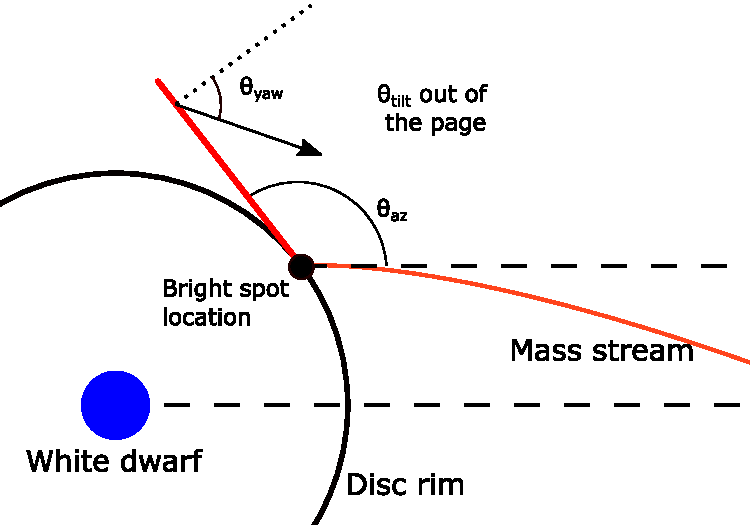
\includegraphics[width=0.7\textwidth]{figures/modelling/bright_spot_schematic.pdf}
    \caption{Showing a schematic of the bright spot model. The {\bf lower dashed line} joins the centres of the white dwarf and donor stars, and the {\bf upper dashed line} runs parallel to it, intersecting the bright spot location. The {\bf straight red line} is one half of the flux-emitting strip and has a profile exponent $Y$, and the {\bf arrow} shows the direction of light emission, at an angle $\theta_{\rm yaw}$ from the normal.}
    \label{fig:modelling:bright spot schematic}
\end{figure}

Lower values of $q$ will cause the ballistic stream to take a wider arc towards the white dwarf, moving the intersection point with the disc. The angle between the bright spot and disc edge is defined by $\theta_{\rm az}$, the angle between the strip and the line of sight of the observer.

As the bright spot is the most complex component of the model, there is an option to simplify it in software for systems with faint bright spot features that cannot be properly resolved.
This mode is called the `simple' bright spot model, and fixes $\theta_{\rm tilt}$ at $90^\circ$, $\theta_{\rm yaw}$ at $0^\circ$, and the strip exponents $X$ and $Y$ to 1 and 2, respectively. By removing these four degrees of freedom, better and faster characterisation of the eclipse is possible.

\subsubsection{Choice of priors}

The choice of prior is important in Bayesian inference, but we have very little prior knowledge on a system. The prior distributions used were generally uniform and span the numerically allowed range\footnote{e.g.\ angles are limited to be between 0 and $2\pi$, and fluxes range from 0 to the peak flux of the eclipses.}, with a few exceptions.

As it is unconstrained by data, $u_{\rm ld}$ initially uses a Gaussian prior centred on 0.3 with a width of 0.1.
The bright spot scale draws from a log-uniform prior between 0 and 0.2, which favours smaller values, and $\theta_{\rm az}$ is forbidden from values that would cause the bright spot strip to deviate from a tangent to the disc by $>80^\circ$.
In addition, some combinations of parameters are forbidden in the model. The values of $q$ and $\Delta\phi$ must be such that $i \leq 90^\circ$ for an eclipse to occur, and the disc radius is constrained by the maximum radius before precession becomes a significant effect, $R_{\rm disc} / a < 0.46$.\todo{REF}


\subsection{Post-processing the eclipse model}
\label{sect:modelling:post processing the eclipse model}

The eclipse modelling uses proxy variables, so some processing must be done to convert them to physical values. This is done in two steps. First, a white dwarf temperature and surface gravity are fit to the white dwarf fluxes. Then, the white dwarf temperature and orbital period are combined with the best-fit eclipse model parameters to convert the scaled distances to metres, and mass ratio to the masses of each star.

\subsubsection{Fitting white dwarf colours}
\label{sect:modelling:fitting white dwarf colours}
By modelling the eclipse in multiple bands, at least three observations of white dwarf flux are available.
The DA white dwarf cooling model from \citet{Bergeron1995}\footnote{Available at \href{http://www.astro.umontreal.ca/~bergeron/CoolingModels}{http://www.astro.umontreal.ca/~bergeron/CoolingModels}} is fit to these flux observations.
These cooling models yield the absolute magnitude of the white dwarf in each band, $M$, for a given effective temperature, $T_{\rm eff}$ and surface gravity, $\log (g)$. This absolute magnitude is then easily translated to an apparent magnitude, $m$, given a system parallax, $\pi$, and interstellar extinction coefficient, ${\rm E(B-V)}$,
\begin{equation}
    m = M - 5\log (\pi\mathrm{,\ arcsec}) - 5
\end{equation}

To optimise these four parameters, an affine-invariant MCMC with three levels of parallel tempering was used, c.f. \S\ref{sect:modelling:parallel tempering}. for priors, uniform $T_{\rm eff}$ and $\log (g)$ distributions were used that span the range set by the model cooling tracks. ${\rm E(B-V)}$ used a uniform distribution between 0, and the maximum IRSA measurement for the relevant sky coordinates\footnote{Available at \href{https://irsa.ipac.caltech.edu/applications/DUST/}{https://irsa.ipac.caltech.edu/applications/DUST/}}, and the parallax prior was chosen to match the Gaia measurement of the system \citep{lindegren2018, Luri2018, Gaia2016, Gaia2018}.

\subsubsection{Conversion of proxy variables to physical parameters}
\label{sect:modelling:conversion to physical parameters}
The eclipse model proxy variables are then converted to real values.
Five input variables are needed: $T_{\rm eff}$, $P_{\rm orb}$, $q$, $\Delta \phi$, and $R_{\rm wd} / x_{l1}$.


A measure of the white dwarf radius, $R_{\rm wd}$, can be found using Kepler's 3rd law and making the substitutions $r = R_{\rm wd} / a$ and $q = M_{\rm donor} / M_{\rm wd}$.
\begin{align}
    P_{\rm orb}^2 &= \frac{4 \pi^2 a^3}{G (M_{\rm wd} + M_{\rm donor})} \\[8pt]
    &= \frac{4 \pi^2 R_{\rm wd}^3}{G M_{\rm wd} (1 + q) r^3} \\[8pt]
    R_{\rm wd}^3 &= \frac{P_{\rm orb}^2 r^3 G M_{\rm wd} (1 + q) }{4 \pi^2}
    \label{eqn:modelling:geometric radius}
\end{align}
$r$ can be found from $R_{\rm wd} / x_{l1}$ by calculating $x_{l1} / a$, which itself is a function only of $q$.

Finding $R_{\rm wd}$ this way requires the white dwarf mass. Fortunately, for a given $T_{\rm eff}$ (which is known from the colour fits, \S\ref{sect:modelling:fitting white dwarf colours}), white dwarfs follow tight theoretical mass-radius relationships \citep{parsons2017}, that can be employed to find the unique $M_{\rm wd},\ R_{\rm wd}$ pair that satisfies both Equation~\ref{eqn:modelling:geometric radius} and the theoretical mass-radius relationship.
Specifically, a proposed theoretical mass-radius pair is chosen from a model relationship and a value of $R_{\rm wd, calc}$ is calculated from Equation~\ref{eqn:modelling:geometric radius}. If this matches the theoretical value, the mass is valid. Otherwise, the proposed mass is altered accordingly and a new mass-radius pair is checked again until the two agree.

Three white dwarf mass-radius relations were used. First, a solution was searched for using the \citet{wood1995} models, spanning masses of $0.4 - 1.0 M_\odot$. The \citet{wood1995} models are preferred, as they use a thicker hydrogen layer that is more appropriate for the accreting CV white dwarfs.
If no solution could be found, the \citet{panei2000} models were searched, spanning masses from $0.4 - 1.2 M_\odot$.
Both of these mass-radius relationships account for the white dwarf $T_{\rm eff}$.
If no solution has been found with these two tracks, the \citet{hamada1961} 0 Kelvin mass-radius relation is checked for solutions. This track spans the largest range in mass, from $0.14 - 1.44 M_\odot$. If no solution is found with the \citet{hamada1961} tracks, the model is considered invalid, though this did not occur for any system in this thesis.

Then, the inclination is calculated. $\Delta \phi$ is solely a function of $q$, and $i$. Therefore, we can use the eclipse model values of $\Delta\phi$ and $q$ to calculate the system inclination - this is done by proposing candidate values of $i$, and comparing the calculated $\Delta \phi_{\rm calc}(q,i)$ with the modelled $\Delta \phi$, and adjusting $i$ as needed until the two agree.

Now, three quantities are known; $i$, $M_{\rm wd}$, and $R_{\rm wd}$. As previously mentioned, $R_{\rm donor}$ is assumed to be the Roche radius, from Equation~\ref{eqn:introduction:eggleton approximation}, and $M_{\rm donor}$ is found simply by $(q \cdot M_{\rm wd})$. $a$ is calculated from the two component masses and $P_{\rm orb}$, using Kepler's laws. Finally, the orbital velocities, $K_{\rm wd,\ donor}$ respectively, of the two stars are calculated using Kepler's laws.
\begin{align}
    K_{\rm wd} &= \frac{2\pi a \mathrm{sin}i}{P_{\rm orb}} \frac{q}{1+q} \\
    K_{\rm donor} &= K_{\rm wd} \cdot \frac{M_{\rm wd}}{R_{\rm wd}}
\end{align}


\subsection{Capturing flickering with Gaussian Processes}

CVs almost always display some amount of stochastic variability, known as flickering. Rather than attempting to model this physically, it is instead treated as correlated noise and characterised with a Gaussian process (GP).
The application of GPs to capturing flickering was established by \citet{McAllister2017} based on work by \citet{roberts2012} and \citet{gibson2012}.
The utility of this addition to the eclipse modelling step is a significant improvement in the accuracy of parameter posteriors, as the GP can be used to subtract flickering from the observations while leaving the key lightcurve features that modelling aims to reproduce, demonstrated by \citet{McAllister2017}.

This section is aimed at giving a working knowledge of GPs in the context of characterising flickering, and for more in-depth discussion the reader is directed towards these works. The mathematics below omits error in flux for legibility, but closely similar derivations are possible that include error when calculating the likelihood of a data set.

\subsubsection{Gaussian Process background}
\label{sect:modelling:GP background}

GPs are a statistical method that can be adapted to produce a series of correlated points across a time (or space) axis, the distribution of which is described by a Gaussian function. The points are related to one another by a joint distribution; to illustrate what a joint distribution is, take the example to two variables $t_1, t_2$, shown graphically in Figure~\ref{fig:modelling:joint distribution}. Each is normally distributed about a central value, but higher values of $t_1$ are more likely to be produced alongside higher values of $t_2$. Thus, knowing the value of $t_1$ can inform the likely value of $t_2$, written as $P(t_1 | t_2)$.

\begin{figure}
    \centering
    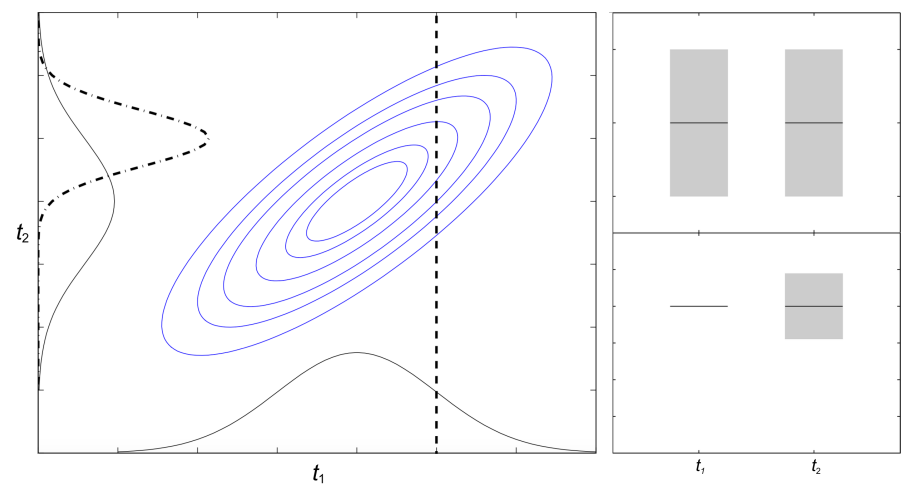
\includegraphics[width=.8\textwidth, clip, trim={0 0 8.5cm 0}]{figures/modelling/joint_distribution.png}
    \caption{Reproduced from \citet{McallisterThesis}. Two variables, $t_{1,2}$, are described by a joint Gaussian distribution. {\bf Blue ellipses} trace lines of equal probability of drawing a sample. {\bf Solid black Gaussians} along each axis show the probability distributions of each variable, and the {\bf dashed black Gaussian} along the y-axis shows the probability distribution of $t_2$, given a fixed value of $t_1$, which is shown by the {\bf vertical dashed line}.}
    \label{fig:modelling:joint distribution}
\end{figure}

By describing a time-series dataset as an arbitrarily large number of variables with a joint distribution between them, the probability of a point being described by a GP, \textit{given the rest of the data}, can be computed. Similarly, the likelihood of an entire data set being described by a GP is also calculable. This principle is the basis of time-series GPs, and allows them to be used when evaluating the goodness-of-fit of a model.

A GP distribution is defined simply by two functions, a mean function, $\mu(t)$, and a covariance function, $k(t_i, t_j)$.
\begin{equation}
    y(t) \sim \mathcal{GP}(\mu(t) \cdot k(t_i, t_j))
\end{equation}
where $t_{i, j}$ are the times of two data points, and are not necessarily adjacent. In this context, the set of $\bf y$ is a set of observed fluxes at times $\bf t$. The distribution of $\bf y$ is then represented by the joint distribution of $P({\bf y} | {\bf t})$, following a multivariate Gaussian, $\mathcal{N}$,
\begin{equation}
    P({\bf y} | {\bf t}) = \mathcal{N}(\mu({\bf t}), {\bf K})
\end{equation}
Where $\bf K$ is the covariance matrix of the multivariate Gaussian, and fully describes how the distribution of each element of $\bf t$ is affected by each other element, forming an $n \times n$ matrix for $n$ data in $\bf t$.
\begin{equation}
    {\bf K} =   \begin{pmatrix}
        k(t_1, t_1) & k(t_1, t_2) & \cdots & k(t_1, t_n) \\
        k(t_2, t_1) & k(t_2, t_2) & \cdots & k(t_2, t_n) \\
        \cdots      & \cdots      & \cdots & \cdots      \\
        k(t_n, t_1) & k(t_n, t_2) & \cdots & k(t_n, t_n) \\
            \end{pmatrix}
\end{equation}

\subsubsection{Computing a covariance matrix}
\label{sect:modelling:GP Kernel choice}

In practice, as $\bf t$ becomes a larger set and $n$ increases, computing the $n \times n$ matrix $\bf K$ becomes impractical. Instead, a kernel is defined that gives analytical functions that approximate each $k(t_i, t_j)$, and the choice of kernel defines the type of correlation between data.

When modelling flickering, a Matern-3/2 kernel is used, which produces a covariance matrix that correlates nearby values more strongly than those further away in time. The kernel has a `memory' timescale, $\lambda$, and an amplitude, $\alpha$, that can be tuned to a data set. This replaces $k(t_i, t_j)$ with $\alpha \cdot k_{M}(r^2)$, where $k_{M}(r^2)$ is defined as
\begin{equation}
    k_{M}(r^2) = \big(1+\sqrt{3r^2}\big) \cdot\exp\big(-\sqrt{3r^2}\big)\ .
\end{equation}
Here, $r^2$ is a pseudo-radius, and is a function of the distance between the two $t_{i,j}$ being considered. Generally, since the Gaussian process technique is applicable to parameter \textit{vectors}, this is written as
\begin{equation}
    r^2 = ({\bf t}_i - {\bf t}_j)^{\top} \cdot \Lambda^{-1} \cdot ({\bf t}_i - {\bf t}_j)
\end{equation}
Note that the choice of the matrix $\Lambda$ defines how other data in a set affect other data, and can be any square matrix of the same width as $\bf t$. For the GP used in this work, a simple $\Lambda$ is used which has $\lambda$ along the diagonal and 0 elsewhere, making $\lambda$ a kernel scale parameter.
In this model each $t_i$ is a single time value, making $\Lambda$ a $1\times 1$ matrix with values of $\lambda$ along the `diagonal' -- functionally, $r^2 = \lambda \cdot {(t_i - t_j)}^2$.

\subsubsection{Evaluating a model fit with a Gaussian process}
\label{sect:modelling:GP model evaluation}

Finally, the $\mathcal{L}$ of a set of ${\bf y}, {\bf t}$ can be calculated given a GP, i.e. $\mathcal{L}(\alpha, \lambda | {\bf y}, {\bf t})$, analogous to $P({\bf y} | {\bf t})$ \citep{rasmussen2006}.
This is the pertinent step to the modelling, as the likelihood function of the data is replaced with the likelihood of the GP.
When evaluating a proposed $\Theta$ in the MCMC, rather than using $\mathcal{L} \propto \mathrm{exp}(-\chi^2/2)$ the likelihood function is replaced with the likelihood of the residuals after observed fluxes have had the eclipse modelled fluxes subtracted, i.e. ${\bf y}_{\rm res} = {\bf y}_{\rm obs} - {\bf y}_{\rm model}$, given an $(\alpha, \lambda)$ pair. This is expressed more clearly algebraically, as
\begin{equation}
    \mathcal{L} = P({\bf y}_{res} | {\bf t}, \alpha, \lambda) = \frac{1}{(2\pi)^{n/2} |{\bf K}|^{1/2}} \exp \bigg(- \frac{1}{2} {\bf y}_{res}^{\top} {\bf K}^{-1} {\bf y}_{\rm res} \bigg)
\end{equation}

One final factor must be accounted for. Flickering appears to be localised to the region of space near the white dwarf, and often reduces in amplitude substantially during the white dwarf eclipse \citep{McAllister2017}.
To capture this in the GP, two kernels are used: one external to the white dwarf eclipse, and one internal to the white dwarf eclipse. Each shares a value of $\lambda$, but has its own freely variable $\alpha$, $\alpha_{\rm out}$ and $\alpha_{\rm in}$.

Overall, the GP adds three new parameters to the eclipse model: $\alpha_{\rm out, in}$ and $\lambda$, which are optimised alongside the eclipse parameters themselves. $\alpha_{\rm out, in}$ use wide, log-uniform priors to prioritise smaller amplitudes. $\lambda$ uses a narrower log-uniform prior, chosen to prevent the timescale from either exceeding the duration of the eclipse, or becoming shorter than the time resolution between data points.
The slightly more complex parameter space that must now be explored, and more computationally expensive evaluation of $\mathcal{L}$, is made up for in a significantly better characterisation of lower quality eclipses \citep{McAllister2017}.



\subsection{Hierarchical model structure}
\label{sect:modelling:optimising eclipse model parameters}

In this thesis, the lightcurve fitting model used by \citet{McAllister2019} is extended, adopting a hierarchical approach to reduce model complexity.

Changes in the disc radius and brightness profile, and bright spot parameters can mean that the same CV has a significantly different eclipse lightcurve at different times, often making it difficult to justify averaging together many eclipses, as features can become smeared out and uninformative. In the worst-case scenario, all 18 parameters would be independently variable for each eclipse, in each band. However, by sharing some parameters between eclipses and bands, this large number of free parameters is slightly reduced, and the posterior of some parameters can be informed by multiple eclipses. \citet{McAllister2017} share $q,\ R_{\rm wd} / x_{l1}$, and $\Delta\phi$ between eclipses, and we broaden that concept by organising the model into a hierarchical structure, a schematic of which is shown in Figure~\ref{fig:modelling:hierarchical_model}.

\begin{figure}
    \centering
    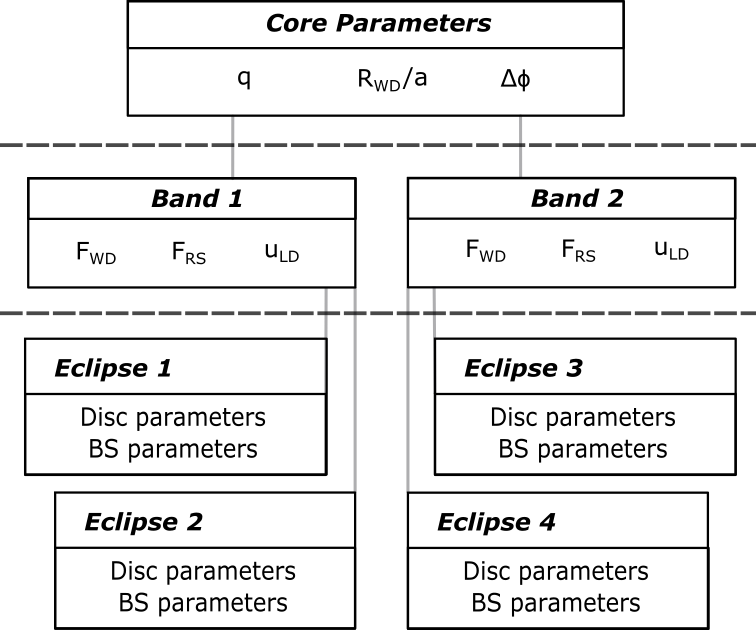
\includegraphics[width=.85\columnwidth ]{figures/results/three_cvs_with_weird_colours/GeneralFigs/hierarchical_model_structure.png}
    \caption{The hierarchical structure of the lightcurve model. Parameters are inherited downwards, to produce an eclipse at the `leaves' of the tree, e.g. Eclipse 3 inherits the parameters of Band 2, which in turn inherits the Core parameters. $\mathrm{F_{WD, RS}}$\ represent the fluxes of the white dwarf and donor star, and $\mathrm{U_{LD}}$\ is the limb darkening coefficient of the white dwarf.}
    \label{fig:modelling:hierarchical_model}
\end{figure}

The top level of the model provides the core parameters, which are unchanging between all observing bands and constant across our observations: $q,\ R_\mathrm{WD}/a$, and $\Delta\phi$. We assume the white dwarf and donor fluxes do not change on the timescale of our observations, and so these variables, along with the limb darkening coefficient of the white dwarf, are shared between all eclipses observed with the same filters. The bottom level holds parameters that can vary quickly enough to change between eclipses, i.e. parameters describing the accretion disc and bright spot. By handling parameters this way, we maximise the amount of data informing important variables. We also somewhat reduce the number of free parameters, which aids in model fitting, but the chief justification for the hierarchical approach is that it ensures consistency between eclipses - something not guaranteed when fitting eclipses individually.

Where possible, data were also binned together. Ideally, this has three beneficial effects: the number of eclipses, and therefore the number of parameters, is reduced; binning increases the signal-to-noise ratio of the data; and as the flickering component is not consistent between eclipses, should reduce the degree of flickering present in the data. However, as CV eclipses often have variable bright spot and disc contributions, it is frequently not reasonable to combine eclipses. Varying bright spot and eclipse features will become smeared out when binned, corrupting crucial elements of the eclipse.
This smearing effect is also subtly present, even in data that are consistent. As a bin width must be chosen that will not precisely align with the integration times of the photometric data, binning will always introduce a small blurring of timing data, and whilst this is a small effect, it can significantly alter the white dwarf ingress and egress features.
Therefore, binning is only done when data are sufficiently similar, and is treated with caution.



\section{Evolutionary modelling}
\label{sect:modelling:evolutionary modelling}

Once armed with a robust sample of CVs donor masses and radii, evolutionary modelling is able to refine our understanding even further. In \S\ref{sect:introduction:Summary of how AML and Mdot drive period evolution}, I motivated how the donor star inflates in response to mass loss, and how the degree of this inflation is related to the severity of the mass loss.
If the radius of an equivalent star in the absence of mass loss is known, and the observed radius of a CV donor can be reproduced by stellar structure models with the introduction of some amount of mass loss, the long-term average mass loss rate can be inferred.

The stellar evolution code used is the MESA codebase \citep{paxton2011,paxton2013,Paxton_2015,paxton2019}, a one-dimensional stellar evolution model. MESA is highly flexible, due to its use of various `modules', wherein each module supplies the code with an element of the physics of the star. These are configurable with relatively simple input files, and can be customised to extend MESA with new physics not contained in the core codebase.
Regarding CV modelling in particular, there is \textit{a priori} cause for confidence; largely default MESA configurations are capable of modelling CV donor tracks with impressive accuracy, even reproducing the period gap by a shutdown of magnetic braking triggered by the donor becoming fully convective \citep{Paxton_2015}.
\S\ref{sect:results:reproducing K11 tracks} also demonstrates this capability, and shows that with some small modifications the agreement between MESA and \citet{knigge11} can be improved further.

Note that all MESA models for this thesis were run using version 21.12.1 of the MESA codebase, and use the configuration detailed in \S\ref{sect:modelling:MESA configs}, unless specified otherwise.

To extract mass loss rates, I will go through three steps.
Firstly, I demonstrate how the radius of a singleton model of a given mass can be tuned to match the M dwarf mass-radius relationship given by \citet{BrownPrep} by introducing star spots, and produce a set of M dwarf models that reproduce observations of stars across the CV donor mass range that \textit{aren't} losing mass.
Secondly, I explore the range of masses for which the radius is a reasonable diagnostic for present-day mass loss rate.
Finally, I outline the method by which I search for mass loss rates that produce stellar models matching CV donor observations.
% Note that all code used for these steps is publicly available online.\todo{But not until Meridith says so!!!!!!}


\subsection{MESA configuration for low-mass M dwarfs}
\label{sect:modelling:MESA configs}

Broadly speaking, when computing a stellar evolution model one must simply input models of physical processes, describe some initial conditions, and allow the stellar model to evolve over time. Unfortunately, the physics of stars in not completely understood, and the processes that affect a star's evolution significantly differ depending on its conditions.
Whilst some core physics is fixed, MESA provides many options for which prescriptions to use for a particular process, or even which processes to consider at all.
MESA has default configuration vales that are reasonable for some common stellar conditions, but some tuning of the model physics is a necessary step for any rigorous modelling.
As such, some tailoring of configuration files must be done in order to produce accurate donor models.

Parameters that are not discussed below are left as the MESA default.
Notably left as default is the metallicity of the donor stars; robust measurements of donor metallicity are challenging, though some recent attempts have yielded results \citep{harrison2016,harrison2018}. However, these are prone to systematic error, and refer to a small sample size. All MESA models presented here assume a solar initial metallicity.


\subsubsection{Model initialisation}

Whilst MESA allows for beginning a MESA run with a precomputed stellar model, the models in this analysis all generate their stars from a pre-main sequence cloud of gas before each run. This ensures that each model is computed from the very beginning with the correct physics, and is set by the command \lstinline{create_pre_main_sequence_model = .true.}


\subsubsection{Nuclear processing}

Computing the equilibrium reaction rates of nuclear burning in a star is non-trivial, as the different species being consumed and produced form a complex network of interactions.
The products of one reaction are often the reagents of another, and with many options for reaction paths and hard-to-calculate reaction rates, this is prohibitive (and often inaccurate) to compute on the fly. Rather, a pre-calculated or empirical reaction network is used.

MESA has several options for the reaction network available in its core codebase. By default, the \lstinline{basic} network considers the reactions of the staple elements of most stellar cores: hydrogen-1, helium-3, carbon-12, nitrogen-14, oxygen-16, neon-20, and magnesium-24.
However, we use the more complete reaction network given by \lstinline{pp_and_cno_extras}. This is a combination of two other networks, \lstinline{pp_extras} and \lstinline{cno_extras}.
\lstinline{pp_extras} is preferred, as it more accurately represents nuclear reactions in young stars \citep{murphy2021}, and \lstinline{cno_extras} more fully considers the reaction chains the CNO cycle, specifically at high temperatures \citep{paxton2011}. To enable this, the lines \lstinline{change_net = .true., new_net_name= `pp_and_cno_extras.net'} are added to the configuration file.

In addition, the JINA Reaclib reaction rate library \citep{cyburt2010} is used: \lstinline{set_rates_preference = .true., new_rates_preference = 2}


\subsubsection{Surface boundary lookup tables}
\label{sect:modelling:MESA surface boundary tables}

When solving the four differential equations necessary to produce an internally consistent stellar model, i.e. how the radius, pressure, luminosity, and temperature vary with mass, some boundary conditions are required.
The boundary conditions for radius and luminosity are self-evident: $R(M = 0) = 0$, and $L(M = 0) = 0$. Unfortunately, such simple fixed central values are not available for the temperature and pressure, so the boundary condition at the surface of the star is used instead.
This requires defining the location of the surface of the star. This is done by setting a value of optical depth, $\tau$, to use as the base of the stellar atmosphere.

A basic approach is to set the pressure and temperature to 0 at the stellar surface, i.e. $P(M = M_\tau) = 0$, $T(M = M_\tau) = 0$, but this is a poor approximation.
A far more accurate approximation is to pre-calculate model stellar atmospheres, which then give values of $P, T$ as a function of $\tau$, $\log(g)$, and luminosity.
Different choices of atmosphere table results in different surface temperatures and pressures, which can alter the mass-radius relation for the resulting models.

For these MESA models, the \lstinline{tau_10} grid was used, which interpolates the PHOENIX \citep{hauschildt1999, hauschildt2001} and \citet{castelli2003} stellar atmospheres (which assume solar metallicity) at $\tau = 10$ for the base of the atmosphere \citep{paxton2010,paxton2011}.
Note that none of the atmosphere tables available in MESA accurately reproduce observations of M dwarfs across the range of donor masses required. In fact, of the available tables, the \lstinline{tau_10} gives some of the less accurate modelled mass-radius relations for low mass stars.
However, this atmosphere grid was chosen as it produces stars that are {\it consistently}\ smaller than required for stars with $M < 0.3 M_\odot$, a deficit that is compensated for in \S\ref{sect:modelling:tuning star spots to observations}, using the method described in \S\ref{setc:modelling:star spot model description}. In this way, rather than relying on the atmosphere table to produce the correct stellar radii, the radius can be manually adjusted to match empirical results.


\subsubsection{Mixing length theory}

Mixing length theory is concerned with the convective boundary, where rising material dissipates its heat, reverses trajectory, and begins to sink.
Models that treat a convective layer as a hard boundary between convective and non-convective material are less able to describe observations than models that allow for some degree of overshooting of rising material past the theoretical convective boundary, before dispersing its energy \citep{prandtl1925}. This is often justified physically by a rising packet of material having some momentum that must be dissipated before reversing direction \citep{bradshaw1974}.

By reducing the degree of overshooting, the efficiency with which energy is transported from the inner regions of the star is similarly reduced, increasing $R(L)$. We decrease the default MESA overshooting of $2\times$ the pressure scale height of the convective boundary, to $1.95\times$ this scale height: \lstinline{mixing_length_alpha = 1.95}. In addition, we use the \citet{henyay1965} MLT formulation, and the following overshooting formalism new to MESA v21.12.1:
\begin{itemize}
    \setlength\itemsep{0em}
    \item \lstinline{overshoot_scheme(:)    = `exponential'}
    \item \lstinline{overshoot_zone_type(:) = `any'}
    \item \lstinline{overshoot_zone_loc(:)  = `any'}
    \item \lstinline{overshoot_bdy_loc(:)   = `any'}
\end{itemize}
% https://docs.mesastar.org/en/release-r21.12.1/reference/controls.html?highlight=overshoot_f#overshooting


\subsubsection{Model convergence and grid fidelity}

Finally, two numerical options were enabled.
The first is the MESA `gold' tolerances, which enforces tight tolerances on energy conservation.
If, after computing a time step, the sum of the energies of each model cell does not closely match the known total energy of the star, the step is rejected and re-attempted, resulting in more accurate models \citep{paxton2019}.
% If a model step has poor residuals, it is rejected and re-attempted, resulting in more accurate models \citep{paxton2019}.

Second, we apply the \lstinline{okay_to_reduce_gradT_excess = .true.} flag, which enables the \lstinline{MLT++} treatment of convection of \S7.2 of \citet{paxton2013}.
When the stellar envelope is superadiabatic and its atmosphere is radiation-dominated, the convective velocities can approach the speed of sound of the stellar envelope. This forces MESA to take extremely short time steps to try and resolve convection, and makes such envelopes prohibitive to model. The \lstinline{okay_to_reduce_gradT_excess} flag allows MESA to reduce the severity of the temperature gradient, making the star less superadiabatic, and less prone to small time steps. This is important to the star spot corrections, as it allows them to be numerically stable for a larger range of spot parameters.


\subsection{Modelling star spots in MESA}
\label{sect:modelling:starspots in MESA}

A general problem in the modelling of low mass stars is an under-estimation of their radii \citep{lopez2005}, and MESA is no exception.
Recently, \citet{BrownPrep}\todo{Get this reference. Can't be long now!} characterised a sample of $\sim 15000$ M dwarfs in detached binaries with a 5th order polynomial, referred to as the Brown relation. We use this empirical mass-radius relation as the baseline `zero mass loss' benchmark radius for comparison against models.

The difference between singleton MESA models with no mass loss and the Brown relation is shown in Figure~\ref{fig:modelling:MESA inflation over Brown relation}, however the goal is not to reproduce the Brown relation exactly; CV donors are filling their Roche lobes, so are non-spherical.
To account for this effect, \citet{knigge11} introduces a $4.5\%$ radius inflation over isolated stars, and I mirror this approach. Thus, the target radius inflation in Figure~\ref{fig:modelling:MESA inflation over Brown relation} is $4.5\%$.
\begin{figure}
    \centering
    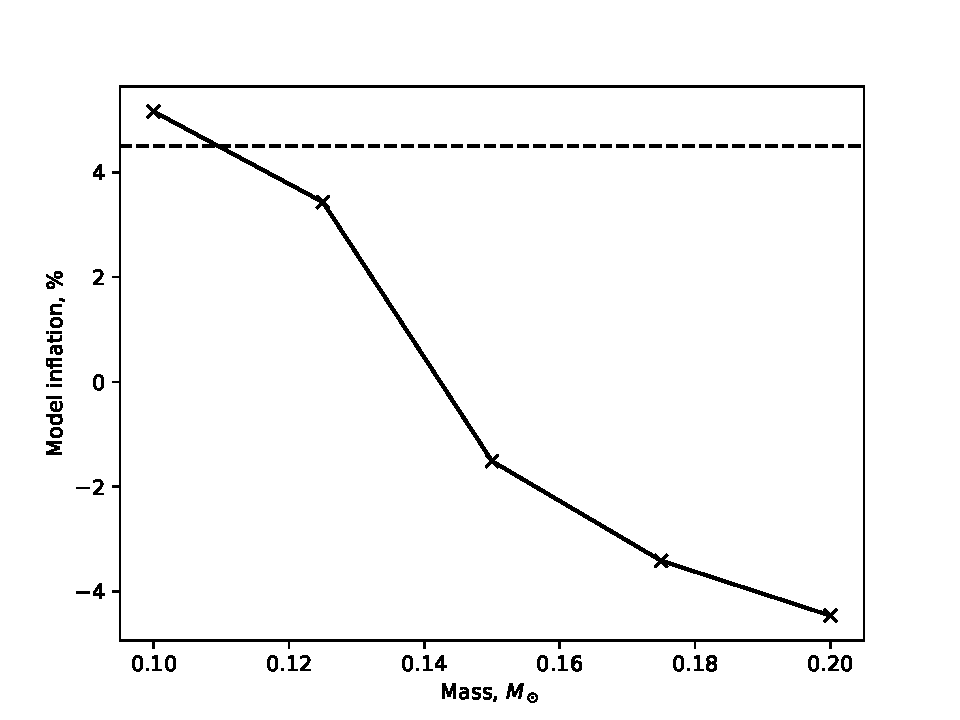
\includegraphics[width=\textwidth]{figures/modelling/MESA_inflation_over_brown.pdf}
    \caption{Showing the radius inflation of default MESA models over the Brown relation, i.e. $(R_{\rm MESA} - R_{\rm brown}) / R_{\rm brown}$. The {\bf horizontal dashed line} is the target radius inflation for MESA models, of 4.5\% over the Brown relation. {\bf Crosses} correspond to MESA models at an age of 2~Gyrs.}
    \label{fig:modelling:MESA inflation over Brown relation}
\end{figure}

To achieve this baseline inflation, I introduce star spots into MESA. Star spots are magnetic phenomena, where the magnetic pressure from concentrations of magnetic field lines provides partial pressure support to the photospheric material, and since spots must remain in pressure equilibrium with the spotted surface, the temperature in a spotted region is reduced by ideal gas laws. As a consequence, the cooler spotted regions emit less black body radiation, inhibiting energy flux out of the stellar interior, and inflating the star.

\subsubsection{The star spot model}
\label{setc:modelling:star spot model description}

As MESA is a one-dimensional code and star spots are a two-dimensional phenomenon, spots are modelled using the formulation given by \citet{sommers2015}, based on work by \citet{spruit1986}.
This implementation was done as a collaboration with Meridith Joyce\footnote{Accreditation} and Marc Pinsonneault\footnote{Accreditation}.

Under this spot treatment, two effects are considered: the photosphere is made inhomogeneous by the presence of spots, and convection is inhibited by the presence of a strong magnetic field.
In the \citet{sommers2015} formulation, the former effect is enforced by altering the effective temperature to a surface-weighted average of the spotted and unspotted surface, and the latter by augmenting the radiative gradient of the star.

The spots cover a fraction of the stellar surface, $f_{\rm spot}$, and a temperature contrast of $x_{\rm spot} = T_{\rm  spot} / T_{\rm amb}$, where the effective temperature of the spotted surface is $T_{\rm spot}$, and the effective temperature of the ambient, unspotted surface is $T_{\rm amb}$. The surface-weighted average of the star, $T_{\rm av}$ is then,
\begin{equation}
    \label{eqn:modelling:surface weighted average temp}
    T_{\rm av}^4 = (1-f) T_{\rm amb}^4 + f_{\rm spot} T_{\rm spot}^4
\end{equation}
And the altered luminosity, $L_{\rm av}$, becomes
\begin{align}
    L_{\rm av} =& 4\pi R^2 \sigma_{boltz} T_{\rm amb}^4 (1 - f_{\rm spot} + f_{\rm spot} \cdot x_{\rm spot}^4) \\
    L_{\rm av} =& 4\pi R^2 \sigma_{boltz} T_{\rm amb}^4 \alpha_{\rm spot} \\
    L_{\rm av} =& L_{\rm amb} \alpha_{\rm spot}
\end{align}
$\alpha_{\rm spot}$, the redistribution parameter, and is what actually alters the structure of the star. $\alpha$ is analogous to the blocking area of perfectly black spots, or spots that are completely supported by magnetic pressure.

MESA performs a lookup for the surface pressure from $T_{\rm eff}$ using precalculated boundary condition tables (\S\ref{sect:modelling:MESA surface boundary tables}). I modify the MESA code to perform this lookup with $T_{\rm av}$.

However, in MESA $T_{\rm eff}$ is not used in the stellar model interior - rather, it uses energies and pressures to calculate structure. Therefore, I alter Equation~\ref{eqn:modelling:surface weighted average temp} to use pressure instead.
Recall the ideal gas equation, for gas in the ambient, unspotted surface, this gas will have pressure and temperature $P_{\rm gas, amb}, T_{\rm gas, amb}$, density $\rho$, and mean molecular weight $\mu$. Here, $R$ denotes the gas constant.
\begin{equation}
    P_{\rm gas, amb} = \frac{\rho R}{\mu} T_{\rm gas, amb}
\end{equation}
The spotted and unspotted surfaces are under pressure
% (and therefore also density\todo{Stu disputes this - send him an email})
equilibrium, but the spotted surface pressure has a contribution from gas pressure, $P_{\rm gas, spot}$, and some contribution from magnetic pressure, $P_{\rm mag, spot}$. Therefore, we can write
\begin{align}
    P = P_{\rm gas, amb} =& P_{\rm gas, spot} + P_{\rm mag, spot} \\
    \frac{\rho R}{\mu} T_{\rm amb} =& \frac{\rho R}{\mu} T_{\rm spot} + P_{\rm mag, spot} \\[12pt]
    P_{\rm mag, spot} =& \frac{\rho R}{\mu} (T_{\rm amb} - T_{\rm spot}) \\
    % P_{\rm mag, spot} =& \frac{\rho R}{\mu} (1 - x_{\rm spot}) T_{\rm amb} \\
    P_{\rm mag, spot} =& (1-x_{\rm spot}) P_{\rm gas, amb} \\
\end{align}
And therefore,
\begin{align}
    P_{\rm gas, spot} =& P_{\rm gas, amb} - P_{\rm mag, spot}\\
    P_{\rm gas, spot} =& P_{\rm gas, amb} - (1-x_{\rm spot}) P_{\rm gas, amb} \\
    P_{\rm gas, spot} =& x_{\rm spot} P_{\rm gas, amb}
\end{align}
However, star spots do not penetrate to the core of the star. To quantify this, rather than fixing $x_{\rm spot}$ and calculating the new pressure at each depth of the star, I calculate the gas pressure differential at the surface of the star, and fix this gas pressure difference for interior layers.
As gas pressure rises with depth, a significant difference at the surface quickly becomes insignificant.
For each depth of the star, $x_{\rm spot}$ is calculated from its total pressure before any alteration is made, $P_i$, and the surface pressure, $P_{\rm surf, amb}$,
\begin{align}
    P_{\rm gas, amb} - P_{\rm mag, spot} =& x_{\rm spot} P_{\rm gas, amb} \\
    x_{\rm spot, i} =& \frac{P_i - P_{\rm surf, amb}}{P_i}
\end{align}
Rather than directly altering the pressure profile of the star, the radiative gradient, $\nabla_r$, at each depth is modified. MESA then uses $\nabla_r$ to compute a self-consistent pressure profile for the star.
\begin{align}
    \alpha_{\rm spot, i} =& 1 - f_{\rm spot} + f_{\rm spot} \cdot x_{\rm spot, i}^4 \\
    \nabla_{r,i}' =& \frac{\nabla_{r,i}}{\alpha_{\rm spot, i}}
\end{align}
Values of $f_{\rm spot}$ and $x_{\rm spot}$ can be passed to MESA as user-configured parameters to define the degree of spotting. Figure~\ref{fig:modelling:spotted model radii at 2Gyrs} shows the radii of main sequence stellar models at 2~Gyrs, and $0.15 M_\odot$ with progressively more spots. The mass-$f_{\rm spot}$ relation required to match the 4.5\% inflation over the Brown relation is searched for in \S\ref{sect:modelling:tuning star spots to observations}
\begin{figure}
    \centering
    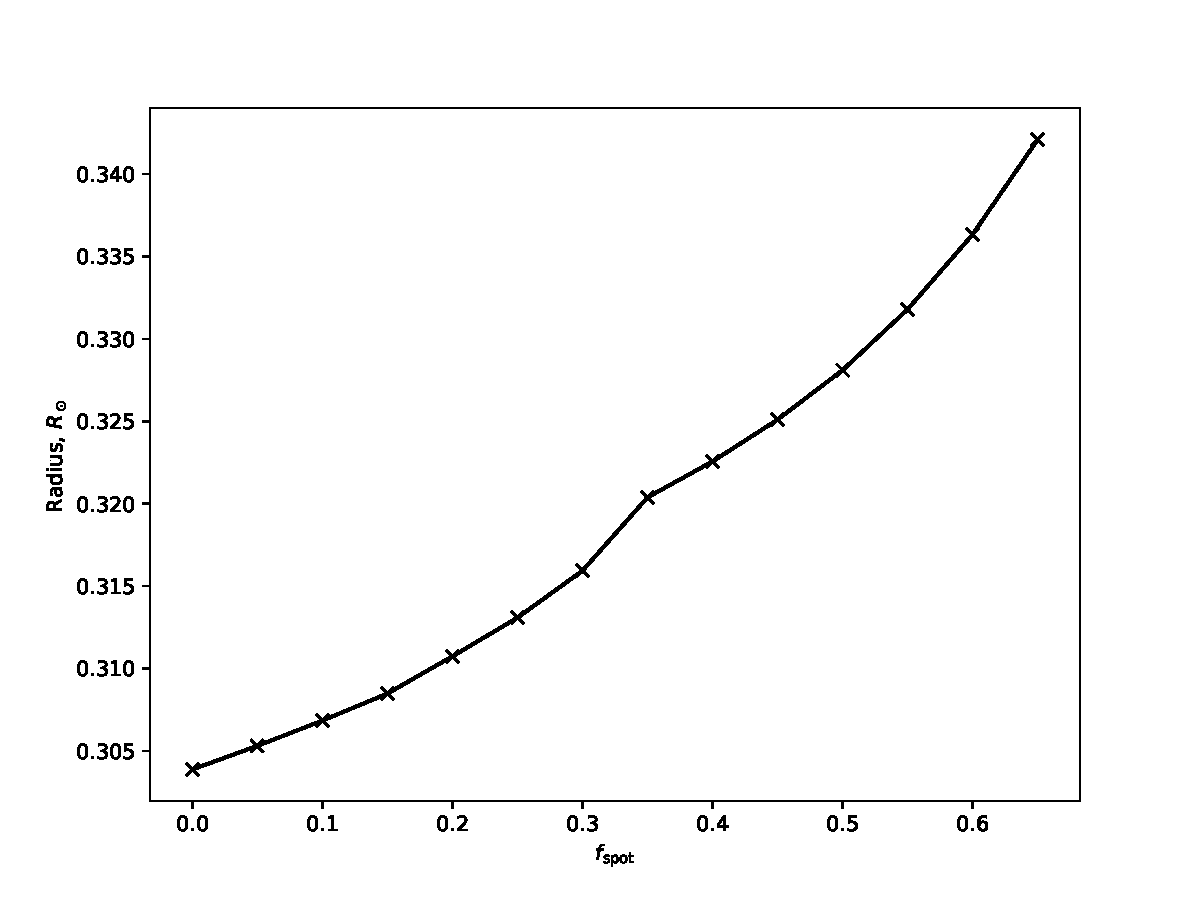
\includegraphics[width=\textwidth]{figures/modelling/spotted_model_radii_at_2gyrs.pdf}
    \caption{Showing how model radius varies as a function of spot coverage for a $0.15 M_\odot$ star. Here, spots are perfectly black ($x_{\rm spot} \equiv 0$), and the radius is extracted at 2~Gyrs. Evaluated MESA models are shown as {\bf black crosses}, and joined by a {\bf black line} to guide the eye.}
    \label{fig:modelling:spotted model radii at 2Gyrs}
\end{figure}


\subsection{Optimising mass loss rate to donor observations}
\label{sect:modelling:optimising mass loss rate to observations}

Finally, the mass loss rate required to match donor observations can be found. As the inflation of the donor increases monotonically with increasing mass loss, the binary chop algorithm is used to precisely and accurately optimise mass loss.
% To sample the error distribution of observed masses and radii, random samples were drawn from the mass and radius posterior distribution for each observation. The mean and standard deviation of the corresponding mass loss rates is reported.

A faster alternative is to run a fixed grid of models, and interpolate within it.
An interpolation grid was constructed with MESA models of fixed $\dot M$ and $f_{\rm spot}$, initialised at a mass of $0.3 M_\odot$. These models were singleton stars, with the configuration described in \S\ref{sect:modelling:MESA configs}. These models were run with fixed values of $f_{\rm spot}$, since varying $f_{\rm spot}$ with mass introduces a time lag between a change in $f_{\rm spot}$, and $R_{\rm donor}$ adjusting that is on a similar timescale to $\tau_{\dot M}$. This effect is demonstrated quantitatively in \S\ref{sect:modelling:tuning star spots to observations}.

Values of $\dot M$ ranged from $-12<\log(\dot M)<-8$ in $\frac{1}{6}$ increments, and $f_{\rm spot}$ spanned from $0<f_{\rm spot}<-0.65$ in increments of 0.05. The initial mass value of $0.3 M_\odot$ was chosen to allow the donor to fully adjust to the $\dot M$-induced inflated radius before reaching the $0.2 M_\odot$ period gap emergence mass.

This results in a grid of model samples in a 4D cube with the axes of mass, radius, $f_{\rm spot}$, and $\dot M$.
For a given $(M_{\rm donor},\ R_{\rm donor})$ pair, a value of $f_{\rm spot}$ can be interpolated from the relationship later derived in \S\ref{sect:modelling:tuning star spots to observations} to choose the correct $f_{\rm spot}$ track, and the model grid can be interpolated for a value of $\dot M$.
This approach is not as accurate as the binary chop optimisation, as the radii from stellar models are not linear functions of the input parameters. However, it is orders of magnitude faster to perform, so is used to characterise the error about a central $\dot M$ value, found with the binary chop algorithm.
% The central value of the binary chop was consistent with the interpolation in all cases.

This mass loss can also be converted to an angular momentum loss rate, assuming none of the mass is retained by the white dwarf. The angular momentum of a binary is given by $J$,
\begin{equation}
    J = M_{\rm wd} M_{\rm donor} \sqrt{\frac{Ga}{M_{\rm wd} + M_{\rm donor}}}
\end{equation}
By differentiating for ${dJ}/{dM_{\rm donor}}$ with the quotient rule, we can find the AML rate by $\dot J = {dJ}/{dM_{\rm donor}} \times {dM_{\rm donor}}/{dt}$. Note that here, I assume the effect of $\dot a$ is negligible, and ignore it (a fuller, more complex treatment of the algebra confirms this -- there is a difference of $\sim 4$ orders of magnitude between the contribution to $\dot J$ from $M_{\rm donor}$ and $a$). Thus, a relation between $\dot M$ and $\dot J$ can be found:
\begin{align}
    \frac{dJ}{dM_{\rm donor}} = M_{\rm wd} \sqrt{Ga} \bigg[ \frac{2M_{\rm wd} + M_{\rm donor}}{2 (M_{\rm wd} + M_{\rm donor})^{3/2}} \bigg] \\
    \dot J = M_{\rm wd} \dot M_{\rm donor} \sqrt{Ga} \bigg[ \frac{2M_{\rm wd} + M_{\rm donor}}{2 (M_{\rm wd} + M_{\rm donor})^{3/2}} \bigg] \label{eqn:modelling:Jdot from Mdot}
\end{align}


\subsection{Mass loss from the white dwarf properties}
\label{sect:modelling:mdot from WD temperature}

The white dwarf temperature also reveals information on the mass transfer rate, and the following summary is described more quantitatively by \citet{townsley2009}.
In brief, as accreted material strikes the surface of the white dwarf its kinetic energy is converted to thermal energy, heating the white dwarf surface.
The degree of this heating is related to the rate at which material falls to the surface -- if more material falls in, more heating is induced.
Since, in general, we can assume that the rate material falls onto the white dwarf is roughly equal to the rate at which material enters the accretion disc from the donor, the white dwarf $T_{\rm eff}$ becomes a diagnostic of the donor $\dot M$.
Simulations demonstrate that even through successive Nova eruptions, the core temperature of the white dwarf is stable over timescales of $\sim 10^8$ \citep{epelstain2007}, so if the accretion rate falls, the white dwarf $T_{\rm eff}$ is able to cool to the appropriate, lower temperature and remain accurate to the present-day accretion rate.

The white dwarf temperature approach holds a major advantage over using the donor properties. Measurements of white dwarf temperatures are easier to gather for large sample sizes.
However, the white dwarf temperature is capable of responding to changes in $\dot M$ on $\tau_{\rm TWD} \sim 10^3 - 10^5\ {\rm yrs}$ \citep{townsley2009}, as opposed to the $\rm \sim~Gyr$ timescales of the evolutionary modelling-based method described above, so only provides a short-term snapshot of the $\dot M$ and is susceptible to corruption from outbursts.
% In addition, the method assumes that the white dwarf is not a helium-core white dwarf, which is not always the case in the CV population and introduces significant unmodelled scatter to the results.

The short-term average mass loss rate, $<\dot M>$, is ultimately a function only of white dwarf mass, and temperature, given in Equation~\ref{eqn:modelling:Mdot from WD temperature}.
\begin{equation}
    \label{eqn:modelling:Mdot from WD temperature}
    T_{\rm eff} = 1.7 \times 10^4 {\rm K} \bigg( \frac{<\dot M>}{10^{-10} M_\odot {\rm yr}^{-1}} \bigg)^{1/4} \bigg( \frac{M_{\rm wd}}{0.9 M_\odot} \bigg)
\end{equation}

Recently, \citet{Pala2021} used spectroscopically measured $T_{\rm eff}$ and $M_{\rm wd}$ to infer the $\dot M$ of 65 CVs, the result of which is reproduced in Figure~\ref{fig:modelling:pala2022 fig13}.
The key finding from this analysis was an inverse correlation between $M_{\rm wd}$ and $\dot M$, contrary to the prediction of gravitational wave braking that lower mass systems should have lower AML rates, driving lower $\dot M$.
As the eclipse modelling of CVs produces a measure of $T_{\rm eff}$, the systems analysed for this thesis can be processed with {\it both} techniques, and have their results compared.
\begin{figure}
    \centering
    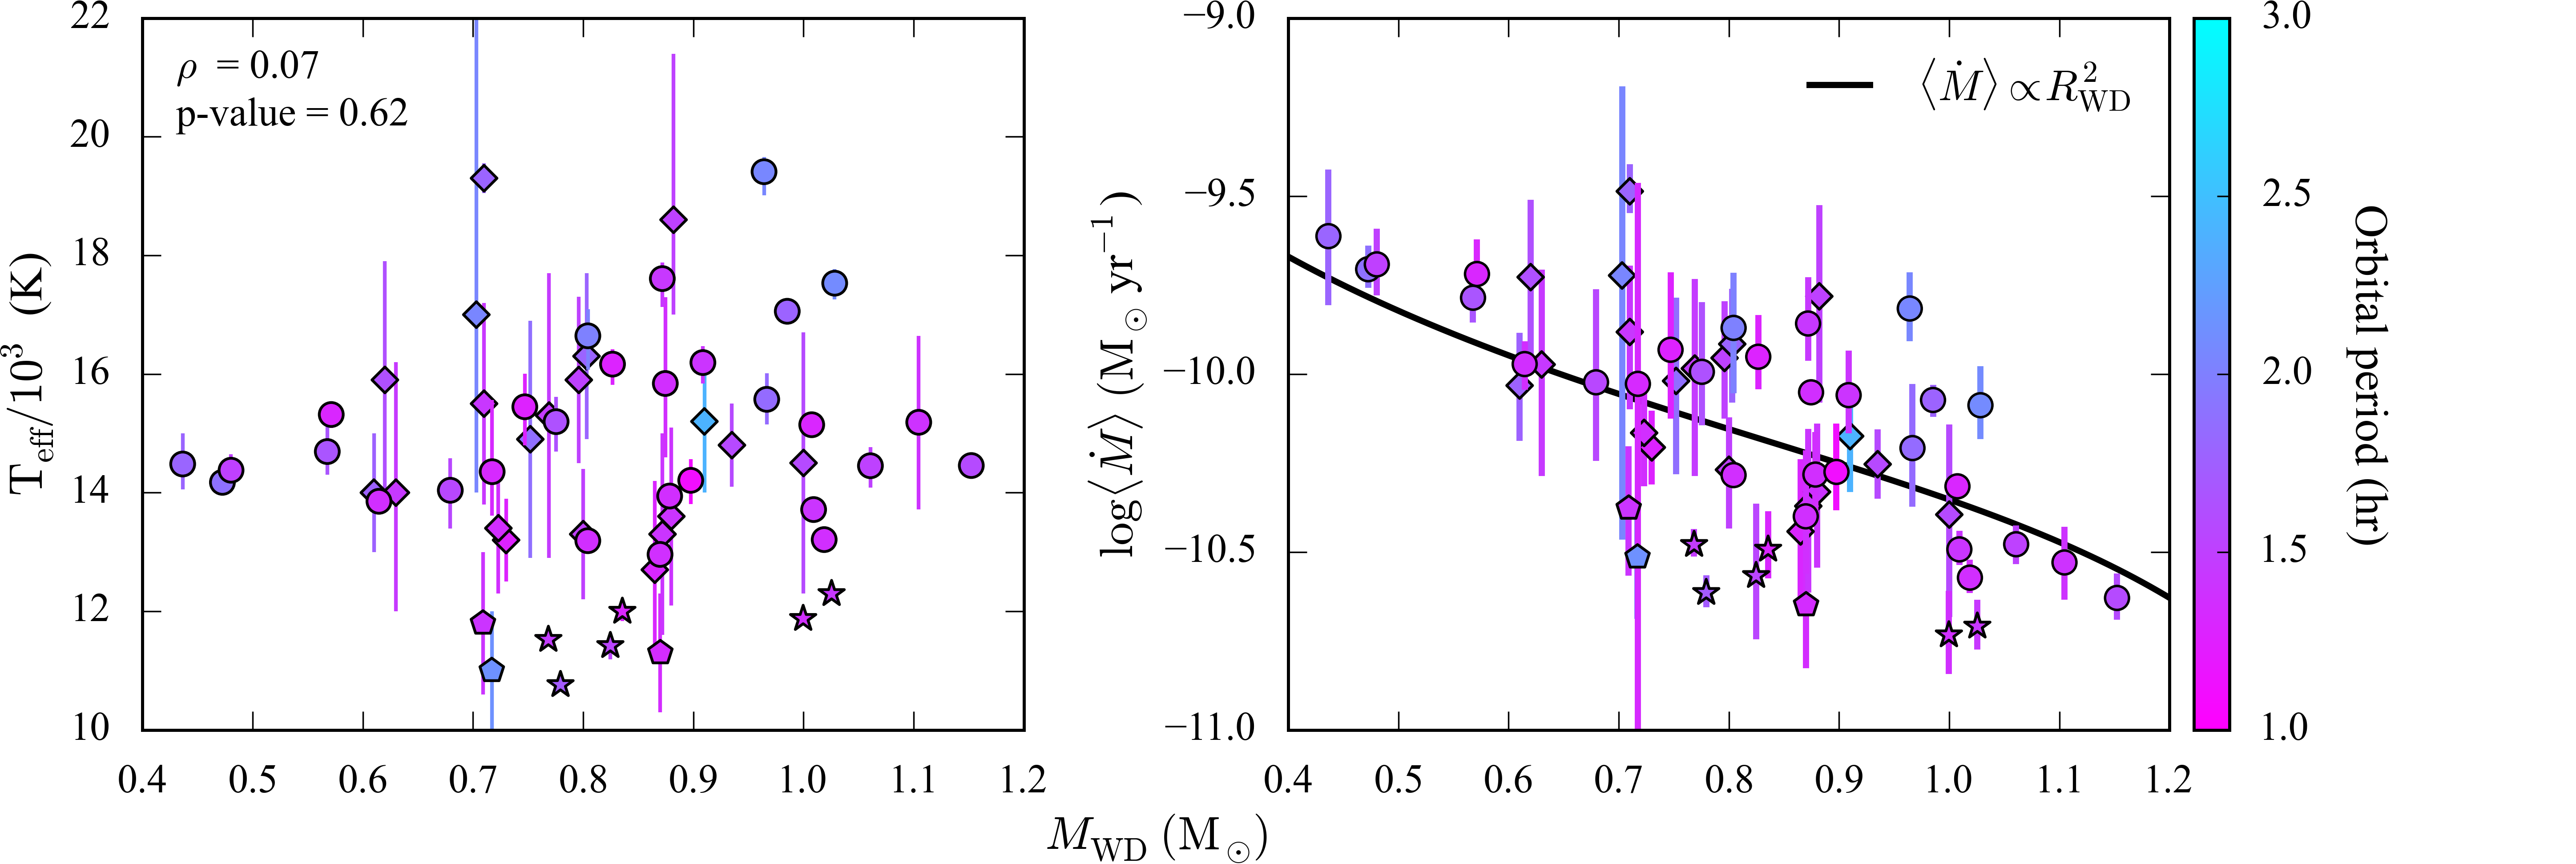
\includegraphics[width=\textwidth]{figures/modelling/pala_2022_fig13.png}
    \caption{Reproduced from \citet{Pala2021}, Figure~13. The subset of modelled systems, with $P < 3{\rm hr}$ are shown. {\bf Circles} and {\bf stars} are pre- and post-period bounce systems derived by \citet{Pala2021}, and {\bf diamonds} and {\bf pentagons} are pre- and post-period bounce systems taken from the literature. {\it Left}: The $T_{\rm eff}$ is plotted against $M_{\rm wd}$, and no correlation can be seen. {\it Right}: $\log<\dot M>$ is plotted against $M_{\rm wd}$, though now the data are correlated along the white dwarf mass-radius relationship assumed by \citet{Pala2021}, $M_{\rm wd} \propto R_{\rm wd}^1.8$. The {\bf black line} shows the rough relationship, and guides the eye.}
    \label{fig:modelling:pala2022 fig13}
\end{figure}
